\subsection{Formulieren} \label{webform}
\pvelist{ \pve{4.24} }

\begin{enumerate}
\item Zorg ervoor dat u bent ingelogd en verzeker u ervan dat u de juiste rechten heeft om resultaten van webformulieren te bekijken.

\item Zoek het formulier op. Een webform is een node, dus u kunt bijvoorbeeld het content-overzicht gebruiken op admin/content en daar filteren op type \emph{Formulier}.

\item Ga naar het formulier en kies de tab \emph{Resultaten}. (Ziet u deze tab niet, dan heeft u onvoldoende rechten. Neemt u in dat geval contact op met uw systeembeheerder).

\item Kies de knop \emph{Downloaden} bovenaan het scherm.

\item Kies als export-formaat \emph{Karaktergescheiden tekst}. Dit biedt de meeste controle op het export-formaat. (De Excel-optie is beperkt en geeft geen werkelijk Excel-bestand).

\item Kies als scheidingsformaat \emph{Sluisteken (|)}. Dit is het meest universele teken, omdat de minste kans bestaat dat dit teken ook voorkomt in de data zelf.

\item Pasoptioneel de extra opties aan.

\item Klik op \emph{Download}.

\item Importeer het bestand in uw spreadsheet-programma (bijv. Excel). Verzeker u ervan dat de import-instellingen juist staan, met name dat ook hier het scheidingskarakter op het pipe-symbool (|) staat.
\end{enumerate}

\subsubsection{Formulieren valideren}
Er zijn regels gemaakt om te valideren wat de gebruiker heeft ingevoerd in het formulier. Deze regels zijn te wijzigen onder het tabblad \emph{Webform} $\Rightarrow$ \emph{Form validation}.

\begin{center}
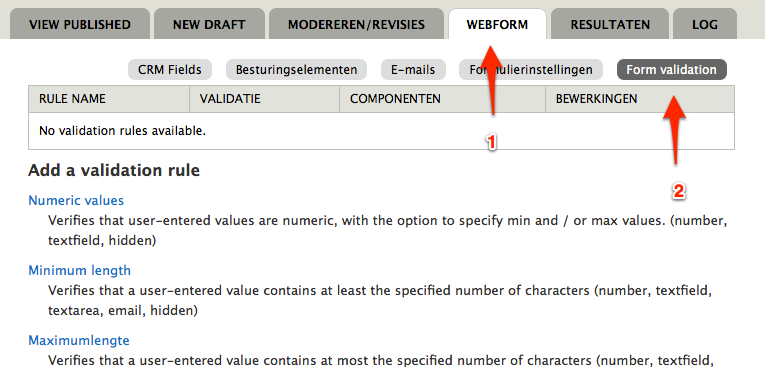
\includegraphics[width=\textwidth]{img/formvalidation.png}
\end{center}

Op deze pagina staat een heel scala aan opties. De volgende zijn met name relevant:
\begin{itemize}
\item Equal values \\
Controleert of de waarde van een veld overeenkomt met de waarde van een ander veld. Dit kan worden gebruikt voor een extra controle op bijv. e-mailadres. Hierbij worden twee e-mail velden aangemaakt. Daarna kan deze regel worden toegevoegt. De regel moet altijd een naam hebben, bijv. \emph{emailcheck} (deze wordt niet getoont aan de gebruiker). Vink daarna de velden aan die gelijk moeten zijn.
\item Regular expression, case insensitive \\
Kan voor diverse doeleinden worden gebruikt. Reguliere expressies zijn een aparte taal dat specifiek voor validatie is bedoeld. Zie verder voor voorbeelden.
\item Regular expression, case sensitive \\
Idem, maar dan hoofdletter gevoelig.
\end{itemize}
Bij de reguliere expressies moeten de volgende gegevens worden opgegeven:
\begin{itemize}
\item Naam, bijv. \emph{postcodecheck} (deze wordt niet getoont aan de gebruiker).
\item Velden waarop de validatie van toepassing is (aanvinken).
\item Regex code (zie verder).
\item Aangepaste foutmelding, bijv. \emph{De postcode is onjuist.}
\item Negate rule: vink deze aan om de regel om te draaien (\emph{mag niet voldoen aan}). In de praktijk wordt deze zelden gebruikt.
\end{itemize}
De regex code bepaald welke invoer valide is. Deze kunnen direct overgenomen worden van de volgende voorbeelden:
\begin{verbatim}
Postcode (Nederlands, met spatie):       ^[1-9][0-9]{3} [A-Z]{2}$
Postcode (Nederlands, zonder spatie):    ^[1-9][0-9]{3}[A-Z]{2}$
Postcode (Nederlands, spatie optioneel): ^[1-9][0-9]{3} ?[A-Z]{2}$
Telefoon (Nederlands vast):              ^0[^6]{1,2}[0-9 \-]{7,10}$
Telefoon (Nederlands mobiel):            ^06[ \-]?[0-9]{8}$
Telefoon (Nederlands mobiel of vast):    ^0[0-9]{1,3}[0-9 \-]{8,10}$
Huisnummer:                              ^[1-9][0-9]* ?[a-z]{,5}.?[0-9]*$
\end{verbatim}
Enkel het stuk van \texttt{\^} t/m \texttt{\$} dient overgenomen te worden.

Voor het valideren van een e-mailadres wordt geen reguliere expressie gebruikt. Er is een type \emph{email} dat gebruikt kan worden als veldtype waar automatisch de goede validatie inzit.

Voor valideren van internationele postcodes is geen reguliere expressie beschikbaar omdat er internationaal geen vast patroon is waar deze aan voldoen. Bij huisnummers moet erop worden gelet dat er uitzonderingen zijn voor bijv. woonboten waarbij "t/o museum" als geldig huisnummer aangemerkt dient te worden. De reguliere expressie houd geen rekening met deze uitzonderingen. Het huisnummer moet hierbij altijd beginnen met tenminste \'{e}\'{e}n cijfer (hoger dan 0), eventueel gevolgd door een letter en evt. weer een cijfer (waarbij spaties gebruikt mogen worden).

Op internet zijn talloze voorbeelden van reguliere expressies te vinden. De site \texttt{regexlib.com} bevat een uitgebreide bibliotheek. Ook via Google zijn deze makkelijk te vinden. Echter zijn er wel meerdere \emph{dialecten}. In Drupal wordt het \emph{Perl} dialect gebruikt (de term \emph{perl compatible} kom je hier weleens tegen). Dit is het meestgebruikte dialect, maar goed testen is altijd van belang!

\subsubsection{Bedankttekst}

\begin{itemize}
\item Bewerk een webformulier
\item Klik op de tab \emph{webformulier}
\item Klik op de subtab \emph{Formulierinstellingen}
\item Voer bij \emph{verzendinstellingen} \emph{Bevestigingsbericht} een bericht in dat getoond wordt na het verzenden van een formulier.
\end{itemize}

\begin{center}
	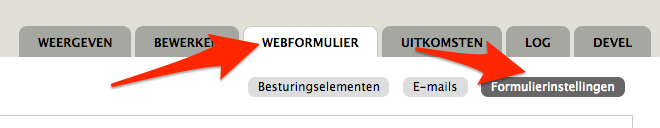
\includegraphics[width=\textwidth]{img/formulierinstellingen.png}
\end{center}

\subsubsection{Verborgen veld}
Bij het aanmaken van een Formulier, kun je nu een veld toevoegen dat niet zichtbaar is aan de voorkant. Dit doe je door te kiezen voor type \emph{Verborgen} en de tekst van \emph{sleutelveld} te laten beginnen met een underscore.

\begin{center}
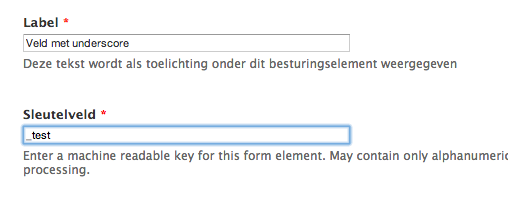
\includegraphics[width=\textwidth]{img/verborgenveld1.png}
\end{center}
Je kunt deze velden nu ook invullen als ingelogde gebruiker in het \emph{gewone} formulier.

Als je dus een besturingselement hebt toegevoegd waarvan het sleutelveld begint met een underscore, zie je dit veld staan bij de inzendingen in de backend.

\begin{center}
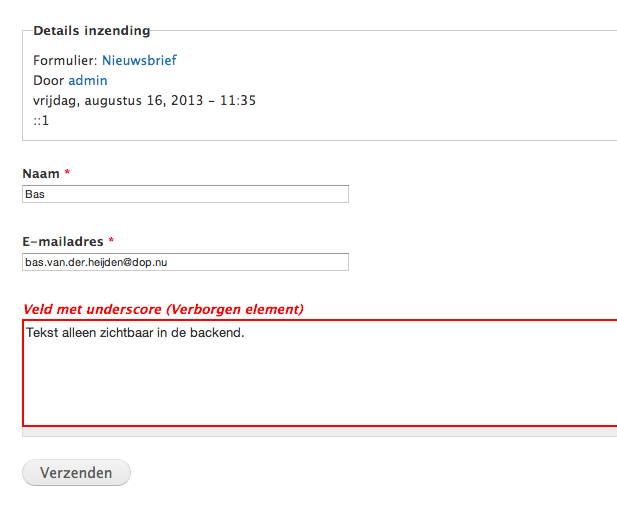
\includegraphics[width=\textwidth]{img/verborgenveld2.png}
\end{center}